\documentclass[conference]{IEEEtran}
\IEEEoverridecommandlockouts
% The preceding line is only needed to identify funding in the first footnote. If that is unneeded, please comment it out.
\usepackage{cite}
\usepackage{amsmath, amssymb, amstext, amsfonts, mathrsfs}
\usepackage{algorithmic}
\usepackage{graphicx}
\usepackage{textcomp}
\usepackage{xcolor}
\usepackage{hyperref}
\usepackage{amsmath}

\def\BibTeX{{\rm B\kern-.05em{\sc i\kern-.025em b}\kern-.08em
    T\kern-.1667em\lower.7ex\hbox{E}\kern-.125emX}}
    
% Kopf- und Fußzeile bearbeitbar machen
\usepackage{fancyhdr}
% Nun gestalten wir die Kopf-und Fußzeile
\pagestyle{fancy}
\rhead{\today}
\lfoot{Mader Mendes Marco \\ Späth Marco \\ Walker Dustin \\}
\cfoot{\thepage}
\rfoot{Signale und Systeme 2 \\  Prof. Dr. Haslach}
\renewcommand{\headrulewidth}{0pt}
\renewcommand{\footrulewidth}{0.4pt}
 
\begin{document}


\title{Signale und Systeme 2 - Praktikum: Abgabe 1}

\author{\IEEEauthorblockN{Mader Mendes Marco}
\IEEEauthorblockA{
\textit{Matrikelnummer: 763153}} % \\
%email address}
\and
\IEEEauthorblockN{Späth Marco}
\IEEEauthorblockA{\textit{Matrikelnummer: 763174}} % \\
%email address}
\and
\IEEEauthorblockN{Walker Dustin}
\IEEEauthorblockA{\textit{Matrikelnummer: 763190}} %//
% matthias.rauscher@student.reutlingen-university.de}
}

\maketitle
\newpage
\pagebreak
\vspace{30cm}


\newpage
\pagebreak
\vspace{30cm}
%
\newpage
\newpage
\newpage
\pagebreak
\vspace{30cm}
\section{Aufgabe 1}
\subsection{Anzahl der benötigten Mikrofonzahl}
\subsubsection{Auswertung mit einem Mikrofonen}
Ein Mikrofon könnte nur den Abstand \textit{r} der Schallquelle zum Mikrofon erkennen. Damit ist keine Positionserkennung möglich, da alle Punkte mit Abstand \textit{r} infrage kommen. 
Alle diese möglichen Punkte bilden eine Kugeloberfläche um den Mittelpunkt (die Position des Mikrofons), mit dem Abstand \textit{r}.

\subsubsection{Auswertung mit zwei Mikrofonen}
Mit zwei Mikrofonen ist eine Eingrenzung der möglichen Positionen der Schallquelle möglich, da nur noch die Schnittmenge der beiden Kugeloberflächen um die Mikrofone als Positionen in Frage kommen. Diese Schnittmenge stellt einen zweidimensionalen Kreisumfang dar. Siehe Abbildung \ref{fig:Normalfall beim Schnitt zweier Kugeloberflächen}. Dieser besteht aber immer noch aus $\infty$ Punkten und ist deshalb im Normalfall nicht geeignet zur Positionsbestimmung. Nur für den Sonderfall, dass die Schallquelle exakt im Mittelpunkt der Geraden zwischen Mikrofon 1 und 2 liegt kann die Position eindeutig bestimmt werden. Siehe Abbildung \ref{fig:Sonderfall beim Schnitt zweier Kugeloberflächen}.
\begin{figure}[b]
	\centering
	\begin{minipage}[t]{0.45\linewidth}
		\centering
		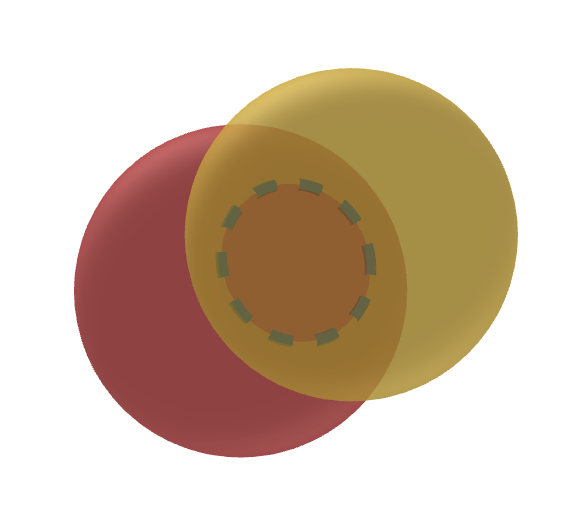
\includegraphics[width=0.75\textwidth]{Schnitt_2_Kugeln}
		\caption{Normalfall beim Schnitt zweier Kugeloberflächen}\label{fig:Normalfall beim Schnitt zweier Kugeloberflächen}		
	\end{minipage}
	\hfill
	\begin{minipage}[t]{0.45\linewidth}
		\centering
		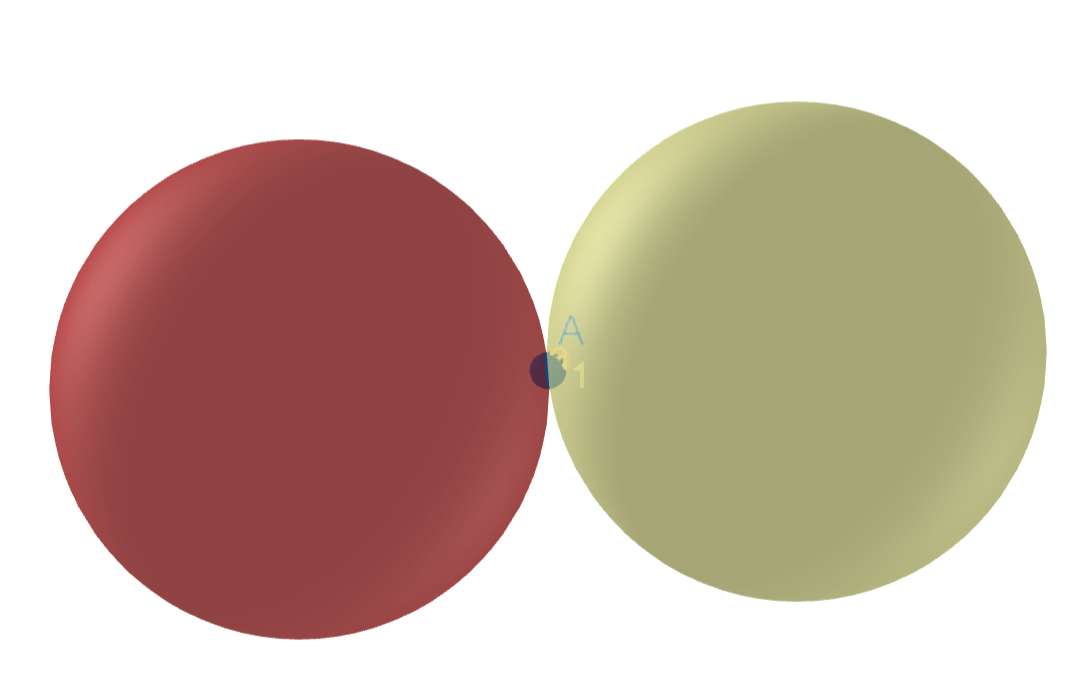
\includegraphics[width=0.75\textwidth]{2KugelnSonderfall}
		\caption{Sonderfall beim Schnitt zweier Kugeloberflächen}\label{fig:Sonderfall beim Schnitt zweier Kugeloberflächen}
	\end{minipage}
\end{figure}

\subsubsection{Auswertung mit drei Mikrofonen}

Durch die Detektion der Schallquelle mit drei Mikrofonen ist die Eingrenzung der möglichen Orte der Schallquelle auf zwei Punkte möglich. Die Orte der drei Schallquellen bilden immer eine Ebene im Raum, es ist nicht möglich, dass sich nur zwei in einer Ebene befinden und das Dritte außerhalb liegt. Darin liegt auch das Problem der zwei Punkte. Einer der beiden Punkte liegt oberhalb der Ebene aus den Mikrofonen mit einem Abstand $\lambda$ zur Ebene. Der Zweite liegt auf einer Geraden, die durch den ersten möglichen Punkt verläuft und orthogonal zur Mikrofonebene ist. Er hat den Abstand -$\lambda$ zur Ebene. Siehe Abbildung \ref{fig:Schnittpunkte dreier Kugeloberflächen}.
Bei der Aufgabenstellung soll ein Raum mit 1m x 1m x 1m Größe nach der Schallquelle durchsucht werden. Wenn die Mikrofonebene in einer der Begrenzungsebenen des Versuchsraums liegt, reichen 3 Mikrofone aus, da der andere Schnittpunkt der möglichen Orte der Schallquelle damit außerhalb des Versuchsraums liegt. Wenn die Mikrofonebene keine der Raumbegrenzungsebenen darstellt, sind drei Mikrofone nicht ausreichend. 
\begin{figure}
\centering 
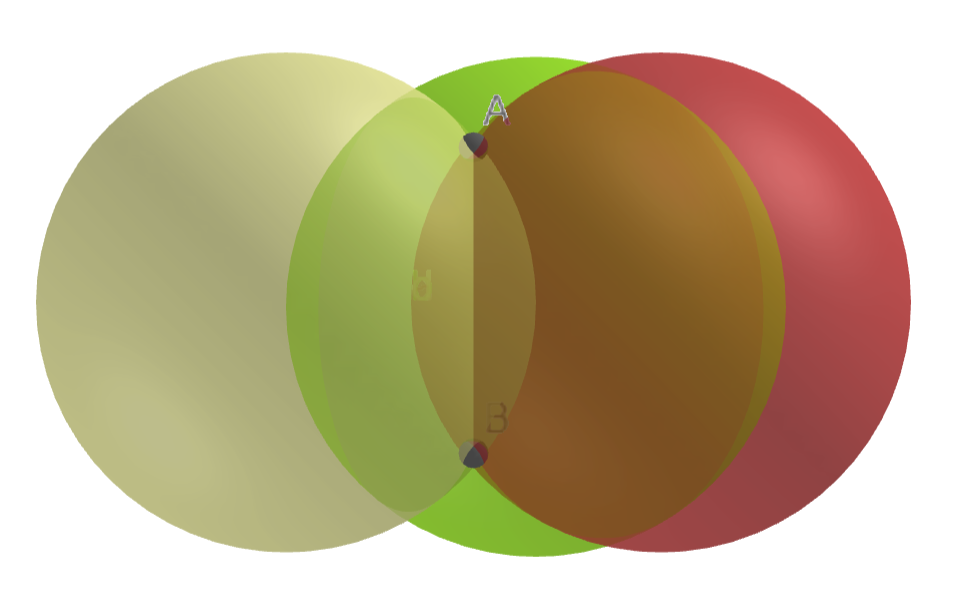
\includegraphics[width=0.4\textwidth]{3Kugeln}
\caption{Schnittpunkte dreier Kugeloberflächen}\label{fig:Schnittpunkte dreier Kugeloberflächen}
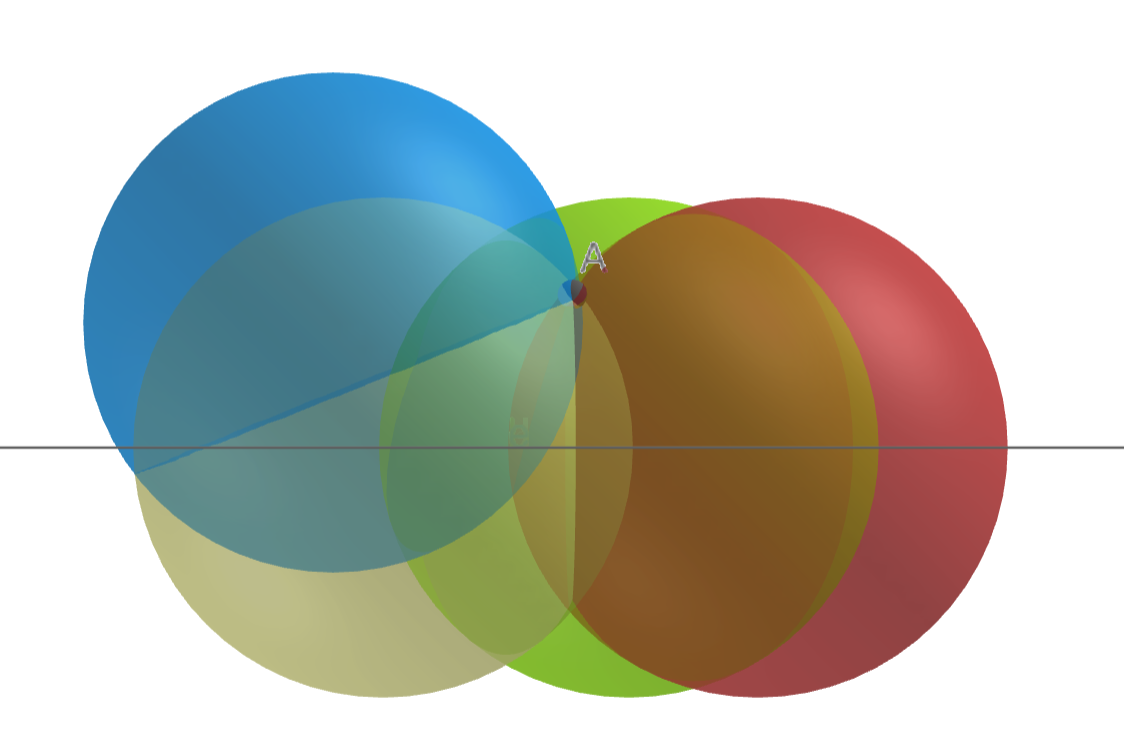
\includegraphics[width=0.4\textwidth]{4Kugeln}
\caption{Eindeutige Schnittpunktbestimmung durch vier Kugeloberflächen}\label{fig:Eindeutige Schnittpunktbestimmung durch vier Kugeloberflächen}
\end{figure}
\subsubsection{Auswertung mit 4 Mikrofonen}
In unserem Fall haben wir nicht die absolute Distanz, zwischen Schallquelle und Mikrofon, sondern nur die Laufzeitunterschiede zwischen den einzelnen Mikrofonen.Im dreidimensionalen Raum benötigen wir drei Informationen. Um drei Laufzeitdifferenzen zu erhalten, benötigen wir vier Mikrofone. 

Wenn sich das vierte Mikrofon nicht in einer Ebene mit den anderen dreien befindet, kann dadurch die Eindeutigkeit des Schnittpunktes zeitgleich garantiert werden. Da damit einer der beiden Schnittpunkte aus dem Fall mit drei Mikrofonen wegfällt. Siehe Abbildung \ref{fig:Eindeutige Schnittpunktbestimmung durch vier Kugeloberflächen}. Für unser Newtonverfahren müssen wir also mit vier Mikrofonen den Versuch aufbauen.



%______________________________________________________________________________________________
\newpage
\pagebreak
\section{Aufgabe 2}
\subsection{Mathematischer Ansatz: Newtonverfahren}
Aus den Zeitverschiebungen, mit der das Signal der Schallquelle von den Mikrofonen aufgenommen wird, kann die Position der Schallquelle im Raum näherungsweise bestimmt werden. Für das Newtonverfahren muss ein erster Ort der Schallquelle geschätzt werden, von welchem aus in mehreren Iterationen der reale Ort der Schallquelle immer besser angenähert werden kann. In einigen Fällen kommt das Newtonverfahren aber zu keinem korrekten Ergebnis. Das ist abhängig von der Positionierung der Mikrofone im Raum, dem Ort der Schallquelle, sowie der Schätzung der ersten Position des Objekts. 

Die Zeitverschiebung der Signale kann durch die Korrelation der Signale S1,S2 und S3 gegen das Signal S0 berechnet werden. Im Buch "Mathematik der digitalen Medien" von Bossert und Bossert wird das Verfahren für den zweidimensionalen Raum sehr ausführlich beschrieben. Weitere Erklärungen zum Verfahren können dort im Kapitel 2.3 unter "zweidimensionale Positionsbestimmung" nachgelesen werden. Auf dieser Arbeit beruhen unsere Berechnungen. Das Verfahren kann sehr leicht auf die hier benötigte, dritte Dimension erweitert werden. Dafür wurde bei den Ausgangsgleichungen eine dritte für die z-Komponente hinzugefügt. Ebenso mussten die partiellen Ableitungen entsprechend von vier auf neun erweitert werden. 
\subsubsection{Ausgangsgleichungen auf drei Dimensionen erweitert}

\begin{align}
\begin{split}
A(x_{n},y_{n},z_{n})  &=  \sqrt{(x_{n}- x_{0})^{2} + (y_{n} - y_{0})^{2} + (z_{n} - z_{0})^{2}} \\& - \sqrt{(x_{n}- x_{1})^{2} + (y_{n} - y_{1})^{2} + (z_{n} - z_{1})^{2}} \\ & - (t_{0} - t_{1}) \cdot v_{0} = 0\label{Gleichung1}
\end{split}
\end{align}

\begin{align}
\begin{split}
B(x_{n},y_{n},z_{n})  &=  \sqrt{(x_{n}- x_{0})^{2} + (y_{n} - y_{0})^{2} + (z_{n} - z_{0})^{2}} \\& - \sqrt{(x_{n}- x_{2})^{2} + (y_{n} - y_{2})^{2} + (z_{n} - z_{2})^{2}} \\ & - (t_{0} - t_{2}) \cdot v_{0} = 0
\end{split}
\end{align}

\begin{align}
\begin{split}
C(x_{n},y_{n},z_{n})  &=  \sqrt{(x_{n}- x_{0})^{2} + (y_{n} - y_{0})^{2} + (z_{n} - z_{0})^{2}} \\& - \sqrt{(x_{n}- x_{3})^{2} + (y_{n} - y_{3})^{2} + (z_{n} - z_{3})^{2}} \\ & - (t_{0} - t_{3}) \cdot v_{0} = 0\label{eq:Gleichung3}
\end{split}
\end{align}

\subsubsection{Partielle Ableitungen der Gleichungen ~\eqref{eq:Gleichung1}}
\paragraph{Ttel}





%________________________________________________________________________________________________#


\subsection{Evaluierung mit zufälligem Fehler $\pm$ $\varepsilon$ }
%_________________________________________________________________________________________________
\subsection{Optimierung der Mikrofonanordnung}

\section{Signalnormierung}
Als ersten Schritt haben wir das Signal des Moskitos Q(t) normiert, um definierte Pegel zu erhalten und ein etwaiges Offset, dass aus der Hardware resultieren könnte herauszurechnen.
\subsection{Mathematischer Ansatz}
Dazu wurde der arithmetische Mittelwert des Signals gebildet und dieser von jedem Signalwert abgezogen. Es wurde nun die Leistung dieses mittelwertfreien Signals berechnet und das Signal mit der Quadratwurzel des Kehrwertes der Leistung
multipliziert. 
In MatLAB kann der arithmetische Mittelwert eines Signals mit der "mean" - Funktion berechnet werden. Die Leistung eines Signals kann mit der "Bandpower" - Funktion berechnet werden.   
\subsection{Gleichung}
\begin{align}
\begin{split}
Q(t) &= dfrac{1}{\sqrt{bandpower(Q(t)- mean(Q(t)))}} \\ &* Q(t)- mean(Q(t))
\end{split}
\end{align}
\section{Mikrofonsignale erstellen}
Um unsere Korrelationsfunktion und die Rauschfilterung zu testen haben wir aus dem bereitgestellten Mosiktosignal die Signale erzeugt, welche von den Mikrofonen aufgezeichnet worden wären. Hierfür haben wir das normierte Signal Q(t) verwendet. \\ 
\subsection{Ausgangssituation}
Die Position des Moskitos im Raum lassen wir uns an einem zufälligen Ort erzeugen. Dieser Ort ist uns aber bekannt. Ebenso berechnen wir uns die Abstände der vier Mikrofone zu dem Moskito. Die Schallgeschwindigkeit vSound ist uns ebenfalls bekannt. Das Soundfile des Moskitos ist uns ebenfalls bekannt aus der Aufgabenstellung. Die Abtastrate des Signals ist uns ebenfalls bekannt und für die Berechnung von Bedeutung\\
Aus der Aufgabenstellung geht hervor, dass die Signale, die von den Mikrofonen aufgezeichnet werden, 100000 Werte beinhalten sollen. Ein Mikrofon mit Abstand 0 zum Moskito soll die Werte 10001 bis 110000 des Moskitosignals aufzeichnen.
\subsection{Berechnung der Mikrofonsignale}
Schalllaufzeit zum Mikrofon :
\begin{align}
\begin{split}
\\ t = \dfrac{Abstand vom Mikrofon zur Schallquelle}{vSound}
\end{split}
\end{align}
Anzahl der verpassten Signalwerte :
\begin{align}
\begin{split}
\\ x = Abtastrate * t
\end{split}
\end{align}
Beginn des Mikrofonsignals:
\begin{align}
\begin{split}
\\ a = Q(10001 + x)
\end{split}
\end{align}
Ende des Mikrofonsignals:
\begin{align}
\begin{split}
 \\b = Q(10001 + x + 100000)
\end{split}
\end{align}

Das kann in MatLAB mit Q(a:b) realisiert werden.
Diese Funktion muss für jedes Mikrofon durchgeführt werden, mit dem entsprechenden Abstand zum Moskito.
So können die vier Ausgangssignale für die weiteren Aufgaben erstellt werden.
\newpage
\section{Aufgabe 2}
Zur Ermittlung der Position des Moskitos wird dessen Fluggeräusch mit vier Mikrofonen gleichzeitig abgetastet.
Dabei wird das Signal mit 48kHz bzw. 96kHz abgetastet. 
Der Empfänger zeichnet gleichzeitig die empfangenen Signale an allen vier Mikrofonen auf. 
Anhand der empfangenen Signalen werden die relativen Laufzeitverzögerungen zwischen den Mikrofonen berechnet und darüber anschließend die Position mit dem bereits erklärten "Newton-Verfahren" ermittelt. Um dabei die Effizienz der Berechnung zu erhöhen, werden die von den Mikrofonen aufgezeichneten Signale gekürzt, diese gekürzten Signale bilden dabei die Hauptsignale. 
Die relativen Verzögerungen werden dadurch ermittelt, dass die Hauptsignale mit einem aus dem Hauptsignal herausgeschnittenen Teilsignal, dem Korrelationssignal, korreliert. Durch die Korrelation eines Teilsignals mit den vier Hauptsignalen lässt sich jeweils die Position des Teilsignals in den Hauptsignalen ermitteln. Anhand der Position lässt sich wiederrum die relative Verzögerung ermitteln. \\
Wie die Signale gekürzt werden, um die wichtigsten Merkmale zu erhalten und dennoch eine beringe Berechnungsdauer gewehrleisten zu können wird im folgenden geklärt.
\\ Zur Vereinfachung werden hier vorerst lediglich die Signale von zwei Mikrofonen betrachtet. 
\subsection{Herrauslösen der Hauptsignale} \label{sec:Eins}
Da die Mikrofone zeitgleich das Signal des Moskitos aufzeichnen, kommt es aufgrund der Laufzeitunterschiede des Signals zu einer Verschiebung der Signalwerte in den empfangenen Signalen untereinander. \\
So empfängt beispielsweise MIC1 den Signalabschnitt $X$ nach 10ms, wohingegen MIC2 aufgrund der größeren Entfernung zum Moskito den selben Abschnitt $X$ erst nach 20ms empfängt.\\
Beginnt man nun beim Herrauslösen der Hauptsignale am Anfang des empfangenen Signals führt dies dazu, dass Mikrofone die näher am Moskito sind diese gar nicht empfangen haben. Dies hat zur Folge, dass die Laufzeitdifferenz nicht korrekt ermittelt werden kann, da die Korrelation keine korrekten Ergebnisse liefern kann.\\
Um diesem Fehlerfall entgegenzu wirken, dürfen die Hauptsignale erst nach einem "Totbereich" herrausgelöst werden. Die Dauer des Totbereiches $t_{min}$ wird dabei über den maximal möglichen Abstand $a_{max}$ der Mikrofone zueinander ermittelt:
$$	t_{min} = \frac{a_{max}}{c_{s}} = 3.57 ms$$
Über die $t_{min}$ und die SamplingRate $f_s$ lässt sich dabei die Größe des Totbereiches $K_{min}$ in der Indexierung des Singales errechnen:
\begin{equation}
	K_{min} = f_s * t_{min}   = f_s * \frac{a_{max}}{c_{s}} \label{eq:A2A2E1}
\end{equation}

Wird der selbe pyramidenförmige Mikrofonaufbau wie im ersten Teil des Praktikums verwendet, ergibt sich für den maximalen Abstand $a_{max}$ eine Distanz von von $a_{max} = \frac{\sqrt{6}}{2}m$. Mit einer SamplingRate von $f_s = 96 kHz$ folgt aus der Gleichung\eqref{eq:A2A2E1} ein Totbereich von $K_{min} \approx 343$. Um noch etwas Sicherheit einzubauen und Rundungsfehler auszugleichen wurde für das Matlab Programm ein Totbereich von $K_{min} = 500$ gewählt.

\subsection{Herrauslösen des Korrelationssignals}
Bei dem Korrelationssignal handelt es sich um einen Auszug aus dem Hauptsignal des ersten Mikrofons welcher als Referenz für die Korrelation mit den Signalen der anderen Mikrofone benutzt wird.\\
Ähnlich wie beim Herrauslösen der Hauptsignale ist auch hier darauf zu achten, dass das Korrelationssignal in den anderen Signalen enthalten ist. Da dies allerdings bereits bei dem Herrauslösen der Hauptsignale berücksichtigt wurde, bildet der erste Teil des Hauptsignal des ersten Mikrofons das Korrelationssignal. Es wird auf eine weitere Verschiebung des Teilsignals verzichtet, um die zu bearbeitende Datenmenge so klein wie möglich zu halten.


\subsection{Länge des Korrelationssignals $K_{corr}$}
Die Länge des Korrelationssignals $K_{corr}$ beieinflusst die Genauigkeit der Differenzmessung deutlich. Ist die Länge des Teilsignals zu kurz, ist keine genaue Positionsermittlung möglich, da es sein kann, dass die betrachteten Wertfolgen mehrmals in dem Hauptsignal auftauchen, bzw. verschwimmen. Durch die Verlängerung des Teilsignals wird dies verhindert und eine exaktere Positionsbestimmung mittels der Korrelation ist möglich. Längere Zeitsignale erhöhen allerdings den Rechenaufwand und damit die Rechendauer. \\
Als Richtwert wird dabei der Extremfall mit der maximal Möglichen Signalverschiebung angewendet. Dieser tritt auf, wenn sich der Moskito auf der Verbindungsgerade der am weitesten entfernten Mikrofone und auserhalb des Raumes befindet. 
Diese maximal Mögliche Signal verschiebung wurde bereits im Unterkapitel \ref{sec:Eins}  errechnet.\\
Somit wird eine Länge des Korrelationssignals von $K_{corr}=350$ verwendet. Die Auswahl wird anhand der Simulation in Unterkapitel  \ref{sec:Untersuchung} genauer untersucht.    
\\
\subsection{Länge der Hauptsignale $K_{sig}$}
Die Länge der Hauptsignale $K_{sig}$ ist direkt von der Länge des Korrelationssignals $K_{corr}$ abhängig. Auch hier ist insbesondere der oben geschilderte Extremfall zubetrachten:\\
Da für eine möglichst exakte Bestimmung ist es notwendig, dass möglichst dass gesammte Korrelationssignal in den Hauptsignalen enthalten ist. Dies ist nur dann der Fall, wenn das Hauptsignal mindestens doppelt so lang ist wie das Korrelationssignal:
\begin{equation}
K_{sig} =  2 * K_{corr}
\end{equation}
Somit ergibt sich für das Hauptsignal eine Länge von 700 Signalwerten.
Durch die Korrelation des kürzeren Korrelationssignal mit längeren Hauptsignalen wird das Zero-Padding reduziert, wodurch eine deutlichere Bestimmung der Laufzeit unterschiede möglich ist.
\subsection{Übersicht der Signale}


\begin{figure}
\centering 
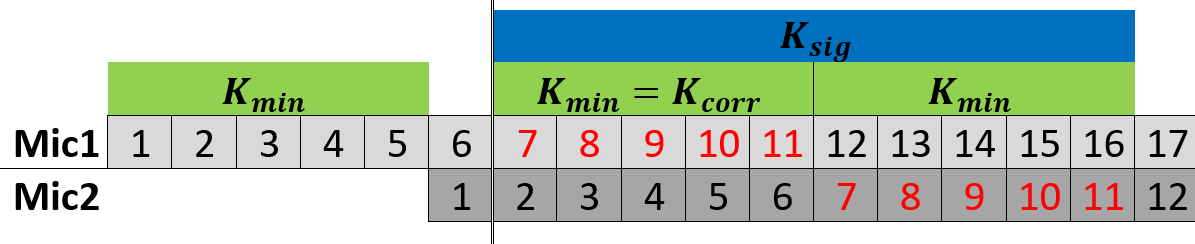
\includegraphics[width=0.4\textwidth]{Korrelation2}
\caption{Signalaufbau, anhand des Extremfalls mit maximaler Signalverschiebung}\label{fig:Korrelation2}
\end{figure}

Der Aufbau der  Signale anhand der genannten Bedingungen ist in Abbildung\ref{fig:Korrelation2} bildlich dargestellt. 
Es wird dabei der Extramfall mit einer maximalen Signalverschiebung (hier 5 ELmente) betrachtet. Würde ein Herrausschneiden der Signale (doppelte Linie) vor dem 5. Element gemacht werden, würden die entsprechenden Signale des zweiten Microfons abgeschnitten werden. Auch eine Verkürzung der Hautsignallänge (blau) würde zu einem Informaitonsverlust führen, da die Betrachtete Korrelationsfolge (rot) nicht mehr komplett im Signal2 enthalten wäre.\\
Oben beschriebene Bedingungen sind in Abbildung sind dann gültig, wenn sich das Moskito in einem Raum der nicht auf den Mikrofonraum von $1m x 1m x 1m$ begrenzt ist befinden kann.
Falls die Begrenzung auf den Mikrofonraums gilt, sollte eine Signallänge von $K_{corr}$ ausreichend sein. Bei der Begrenzung sind obige Bedingungen allerdings nicht hinderlich, sie sollten sogar zu einer höhren Genauigkeit führen. Daher wurden obige Bedinungen gewählt um den Raum des Moskitos zu erweitern.


\subsection{Untersuchung der Annahmen} \label{sec:Untersuchung}
Bei der Untersuchung der erstellten Annahmen stellte sich heraus, dass die Annahmen zu einer sehr hohen Fehlerquote bei der Korrelation führten. Ein Fehler tritt auf, wenn die über das Korrelationsmaximum ermittelte Signalverschiebung nicht mit dem tatsächlichen Wert übereinstimmt. \\

\begin{figure}
\centering 
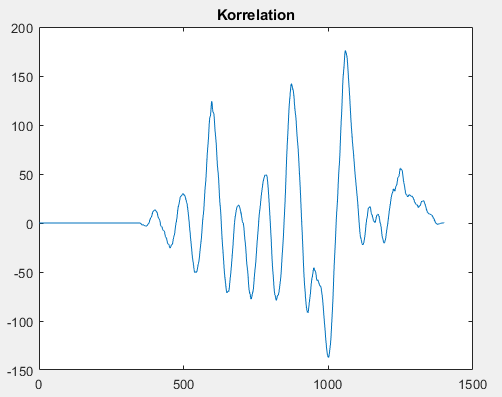
\includegraphics[width=0.4\textwidth]{KorrelationA}
\caption{Beispiel einer "fehlerhaften" Korrelation ($K_{corr}=350$}\label{fig:KorrelationA}
\end{figure}



Sieht man sich die Ergebnisse einer fehlerhaften Korrelation (siehe Abbildung \ref{fig:KorrelationA}) genauer an, fällt auf, dass kein eineindeutiges Maximum auftritt, sondern mehrere. Dabei ist das Problem, dass die "richtigen" Maxima teilweise geringere Amplituden haben als die "falschen". Dies hat zur Folge, dass eine Rechenumgebung ohne die Kenntniss der tatsächlichen Signalverschiebung teilweise falsche Ergebnisse ermitteln wird.\\
Untersucht man das Originalsignal des Moskitos (siehe Abbildung \ref{fig:KorrelationAnalyse2}) genauer fällt auf, dass das Signal eine leichte Periozität aufweist, wobei die Periodendauer des Signals ähnlich des errechneten $t_{min}$ ist. Diese Tatsache erklärt warum es bei der durchgeführten Untersuchung zu mehrern Maxima bei der Korrelation kam. \\
Zur Minimierung der Fehlerquote werden nun verschiedene Paramter untersucht

\begin{figure}
\centering 
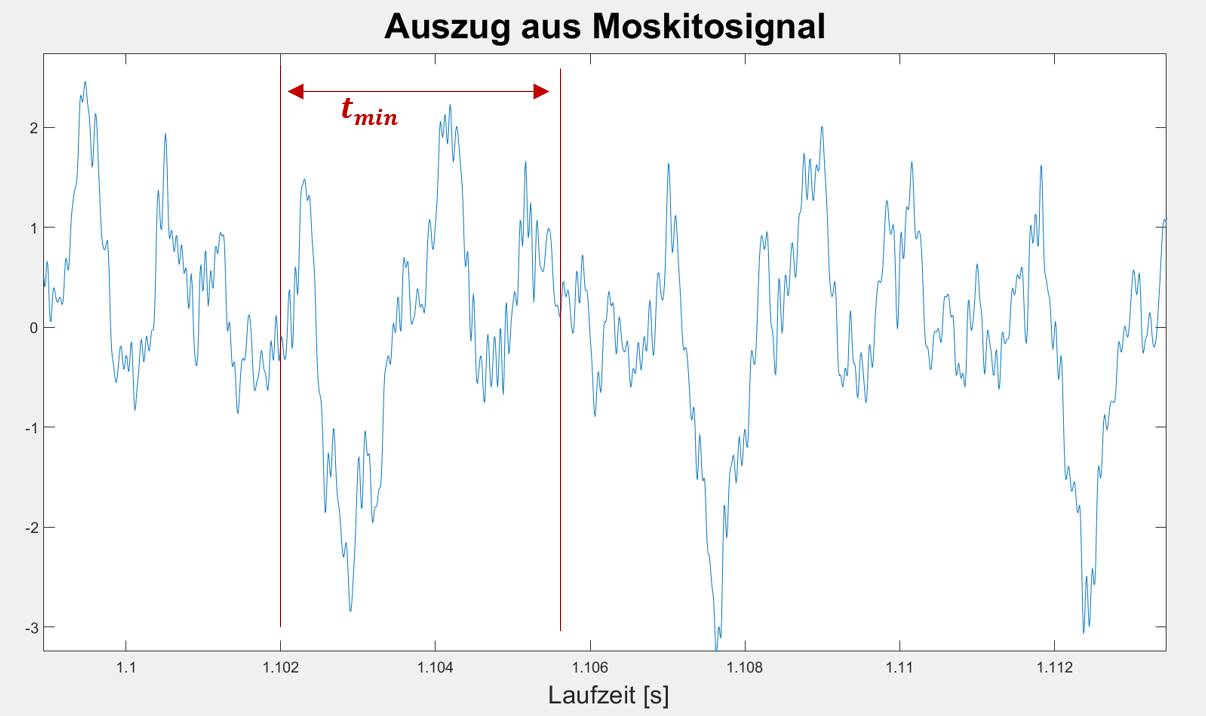
\includegraphics[width=0.4\textwidth]{KorrelationsAnalyse2}
\caption{Auszug aus dem Moskitosignal} \label{fig:KorrelationAnalyse2}
\end{figure}

\subsubsection{Länge des Korrelationssegments}

Die Betrachtung der Korrelationsergebnisse verdeutlicht, dass die errechnete Länge des Korrelationssegments zu kurz ist. Dies wurde dadurch deutlich, dass bei der Ermittlung der Korrelationswerte mehrere Maxima auftraten, da die Korrelationssegmente an mehrereren Stellen im Hauptsignal Ähnlichkeiten aufwiesen. Verlängert man das Korrelationssegment muss zwar mehr Rechenaufwand in Kauf genommen werden, allerdings nimmt auch die Wahrscheinlichkeit ab, dass man ähnliche Teile in den Hauptsignalen findet.\\


\begin{figure}
\centering 
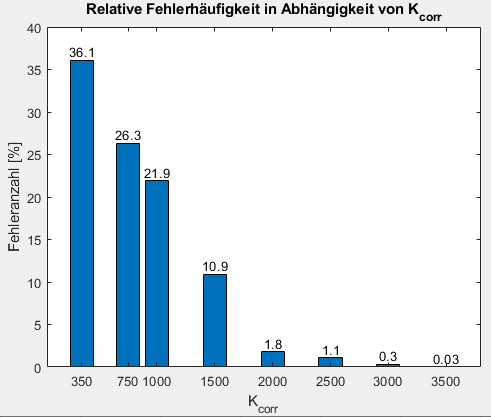
\includegraphics[width=0.4\textwidth]{KorrelationsAnalyse1}
\caption{Relative Fehlerquote in Abhängigkeit von $K_{corr}$  \linebreak(Start der Aufzeichnung nach 10000 Werten)} \label{fig:KorrelationAnalyse1}
\end{figure}

Bei der Analyse wurde die Korrelation mit allen Mikrophonen jeweils 1000 mal durchgeführt und die mittlere Fehlerquote ermittelt. Betrachtet man die Ergebnisse der Analyse (siehe Abbildung \ref{fig:KorrelationAnalyse1}) wird deutlich, dass die Fehlerquote mit zunehmender Länge von $K_{corr}$ abnimmt. Es wird deutlich, dass bei einer Korrelationslänge von 3500 Werten nur noch eine Fehlerquote von $0.03$  Prozent  erreicht wird. Mit einer weiteren Erhöhung könnte man die Fehlerquote weiter senken, allerdings würde dies die Laufzeit weiter verlängern. Betrachtet man die benötigte Laufzeit für 3500 Werte gemäß Gleichung \ref{eq:A2A2E1} wird deutlich, hierführ bereits $36.5ms$ benötigt werden.
Aufgrund des in Abbildung \ref{fig:Korrelation2} beschriebenen Signalaufbaus wird allein eine Signalmesslaufzeit von beinahe $110ms$ benötigt, wobei die benötigte Rechenzeit noch nicht berücksichtigt wurde.
Da eine noch längere Messung das Orten des Moskitos unmöglich machen, da jenes nach der Berrechnung stets an einem anderen Ort sein würde. Sollte keine größere Korrelationslänge als $K_{corr} = 3500$ gewählt  und stattdessen lieber die angegebene  Fehlerquote in Kauf genommen werden.


\subsubsection{Position des Hauptsignals}
Ein weiterer Faktor beim Signal aufbau ist der Beginn der Hauptsignale. Bei der Untersuchung dieses Parameters (siehe Abbildung \ref{fig:KorrelationAnalyse3}) sticht deutlich der Signalstart bei 7500 herraus, da dort die relative Fehlerquote am geringsten ist.
Wiederholt man nun die Analyse aus dem vorherigen Kapitel sind ist hier ebenfalls eine deutliche Verringerung der Fehlerquote zu erkennen (siehe Abbildung \ref{fig:KorrelationAnalyse4}). Auch hier wird deutlich, dass die Fehlerquote mit steigender Länge des Korrelationssignals sinkt.
\begin{figure}
\centering 
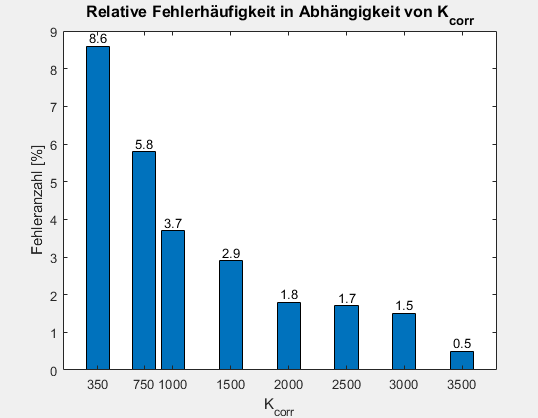
\includegraphics[width=0.4\textwidth]{KorrelationsAnalyse4}
\caption{Relative Fehlerquote in Abhängigkeit von $K_{corr}$  \linebreak(Start der Aufzeichnung nach 7500 Werten)} \label{fig:KorrelationAnalyse4}
\end{figure}

\begin{figure}
\centering 
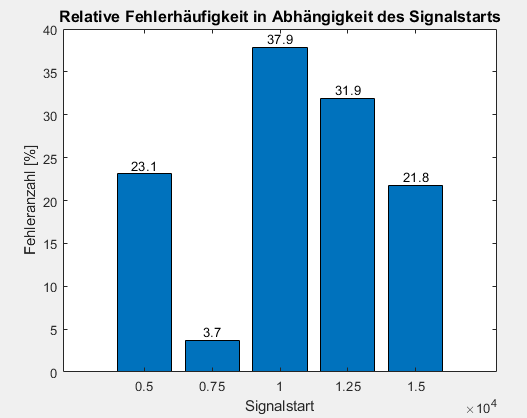
\includegraphics[width=0.4\textwidth]{KorrelationsAnalyse3}
\caption{Relative Fehlerquote in des Signalstarts $K_{corr}$  \linebreak(5000 Messungen mit $K_{corr}=1000$)} \label{fig:KorrelationAnalyse3}
\end{figure}
\subsubsection{Zusammenfassung der Untersuchung }
Abschließend lässt sich zusammenfassen, dass die berechenete Länge des Korrelationssignal deutlich zu kurz für eine akzeptable Positionsbestimmung ist. Aus der Analyse des Startwartes wird deutlich, dass die Ergebnisse stark von dem jeweiligen Signalabschnitt abhängen. Da es in der Realität das Signal des Moskitos allerdings nicht statisch ist wie in der Simulation, ist diese Analyse sekundär, da die Position beim realen Signal nicht beeinflusst werden kann. Allerdings lässt diese Position gut für die Analyse des Rauscheinflusses verwenden. \\\\\\
Für weitere Berechnungen werden von nun an die Parameter wie folgt gewählt:\\
$$K_{Startwert} = 7500$$
$$K_{corr} = 3000$$
$$K_{sig} = 6000$$

\subsection{Korrelation mit awgn Rauschen }
Bis jetzt haben wir angenommen, dass das Audiosignal auf dem Weg von der Signalquelle zum Mikrophon nicht gestört wird. Nun betrachten wir den Fall mit Rauschen. Es werden nur zwei Microphone betrachtet, um das System zu vereinfachen. Wir gehen davon aus, dass wir ein Additive White Gausian Noise (awgn) haben. Dabei handelt es sich um ein Normalverteiltes Zufallssignal mit unendlicher Bandbreite, welches auf unser Nutzsignal aufaddiert wird. Dabei ist das Rauschen auf dem Weg zu Mikrofon 1 unabhängig vom Rauschen auf dem Weg zu Mikrofon 2. Wir wollen nun untersuchen wie dieses Rauschen unser Korrelationsergebnis beeinflusst. Wichtig hierbei ist das Signal to Noise Ratio. Dies beschreibt das Verhältnis der Leistungen vom Nutzsignal zum Rauschsignal. 
$$ snr = \frac{P_{nutzsignl}}{P_{Rauschsignal}} [dB]$$
Mit Hilfe eines Matlab Scripts haben wir simuliert wie sich awgn Rauschen auf die Korrelation auswirkt. Wir haben die Korrelation jeweils 1000 mal für unterschiedliche snr durchlaufen lassen. Die Position der Signalquelle war jedes mal zufällig. Auf dem Schaubild (siehe Abbildung \ref{fig:KorrelationAnalyseMitRauschen}) ist zu sehen, dass wir bis zu einem snr von 7dB eine Fehlerquote von 0\% haben. Bei einem snr von 0dB bzw. 1/1 haben wir gerade einmal eine Fehlerquote von 3\%.




\begin{figure}
\centering 
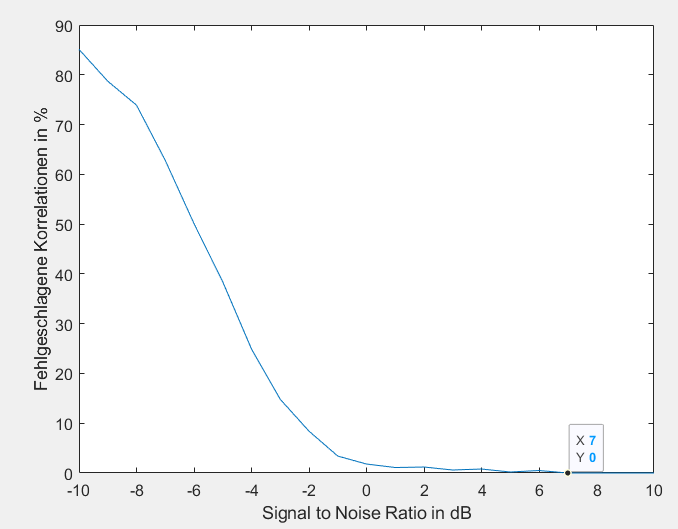
\includegraphics[width=0.49\textwidth]{Correlation mit Rauschen, (SNR) bei 4000 Segmentlaenge und 7500 corrBegin (in dB)}
\caption{Korrelation mit Rauschen} \label{fig:KorrelationAnalyseMitRauschen}
\end{figure}

\subsection{Korrelation mit awgn Rauschen im Dreidimensionalem}
Was bedeutet diese Erkenntnis für unseren Dreidimensionalen Fall mit vier Mikrophonen? Dieser Frage wollen wir uns nun stellen.

\subsubsection{Annahme}
Im Dreidimensionalen muss die Korrelation drei mal pro Positionsbestimmung durchgeführt werden mic1, mic2 und mic3 werden jeweils mit mic0 korreliert, um die Laufzeitdifferenzen zu bestimmen. Wenn man davon ausgeht, dass die Erfolgsquote der drei Korrelationen unabhängig voneinander ist sollte sich die Wahrscheinlichkeit für eine erfolgreiche Korrelation kubieren. Wenn zum Beispiel die Erfolgschancen für eine Korrelation 97\% ist, dann ist die Wahrscheinlichkeit für drei aufeinanderfolgende erfolgreiche Korrelationen $0.97^{3} = 0.913$. Es ist also sehr wichtig, dass eine einzelne Korrelation recht zuverlässig ist.

\subsubsection{Simulation}
Um dieses System zu simulieren haben wir nun die Zeitdifferenzen aus den drei Korrelationen in das Newton Verfahren gegeben um eine berechnete Position der Signalquelle zu erhalten. Für die Simulation haben wir uns für eine Korrelationslänge von 4000 und ein Signal to Noise Ratio von 0 dB entschieden. 
In diesem Prozess können nun zwei mögliche Fehler auftreten. Wenn bei der Korrelation der Falsche Hochpunkt gewählt wird, dann Resultiert das in einem berechnetem Punkt der Schallquelle, welcher meist weit außerhalb des möglichen Raumes. Es ist, wie im ersten Praktikumsversuch schon beschrieben, auch möglich, dass das Newtonverfahren keine Nullstelle findet.




\begin{figure}
\centering 
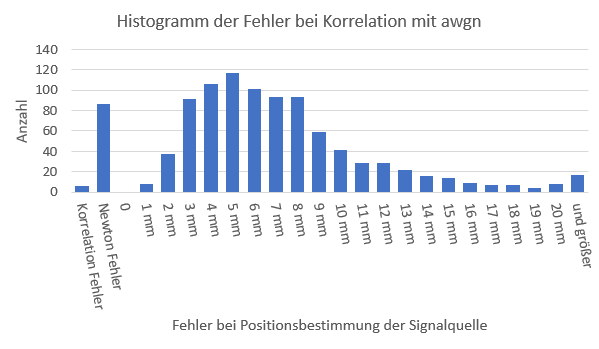
\includegraphics[width=0.49\textwidth]{Korrelation mit Rauschen im Dreidimensionalem, Histogramm zu 1000 Simulationen}
\caption{Korrelation mit Rauschen im Dreidimensionalem, Histogramm zu 1000 Simulationen} \label{fig:KorrelationAnalyseMitRauschen Histogramm}
\end{figure}


\subsubsection{Interpretation des Ergebnisses}
Bei den von uns bestimmten Parametern und dem willkürlich auf 0 dB festgelegtem SNR hat das Moskito noch etwas Überlebenschance. jedes zehnte mal schießen wir komplett daneben. Falls die Korrelation und das Newton verfahren erfolgreich waren, sind wir auf ungefähr 5 mm genau. Ein durchschnittliches Moskito ist 6 mm lang und 2 mm breit. Wir werden also häufiger daneben schießen, als wir treffen. Dies ist jedoch in Ordnung, da wir nur einmal treffen müssen.

\newpage
\pagebreak
\vspace{30cm}
\end{document}